Clusteralgorithmen wirken dem Problem hoher Autokorrelationszeiten im Bereich des Phasenübergangs entgegen.\\
Um dies zu erreichen arbeiten sie nicht mehr nur Lokal, wie der Metropolis Algorithmus, sondern bilden größere Bereiche (Cluster), die auf einmal manipuliert werden.

\subsection{Wolff-Algorithmus}
Der Wolff-Algorithmus ist ein Cluster-Algorithmus, der pro Monte-Carlo-Schritt von einem zufälligen Startpunkt aus ein Cluster bildet und dann mit einer bestimmten Wahrscheinlichkeit alle Spins innerhalb des Clusters flippt.\\
Allgemeiner Programmablauf:\\
1. Startkonfiguration (Abbildung 4.1)\\
2. Bestimmte einen zufälligen Startpunkt (Abbildung 4.2)\\
3. Ausgehend vom Startpunkt werden benachbarte Atome mit gleichem Spin mit Wahrscheinlichkeit p in den Cluster aufgenommen (Abbildung 4.3a,b,c)\\
4. Flippe alle Spins des Clusters mit einer Wahrscheinlichkeit (Abbildung 4.4)\\
5. Gehe zu 1.\\
\begin{figure}[htbp]
  \centering
  \begin{minipage}[b]{6 cm}
    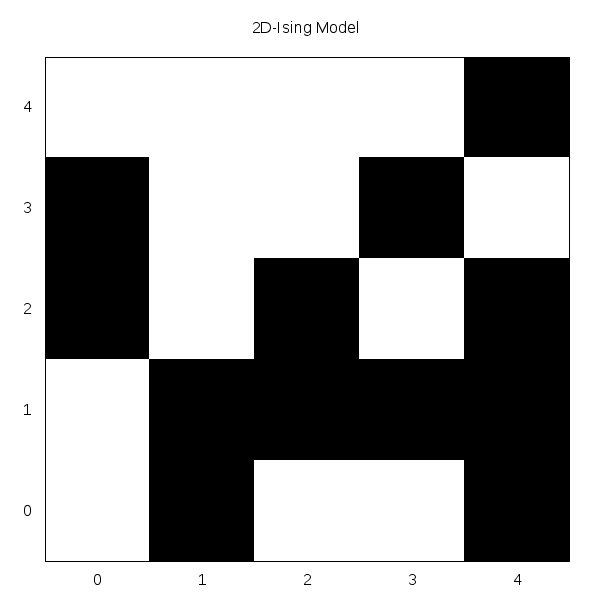
\includegraphics[width=0.5\textwidth]{../Graph_Export/cluster_veranschaulichung/Abbildung41.png}
    \caption{}
  \end{minipage}
  \begin{minipage}[b]{6 cm}
    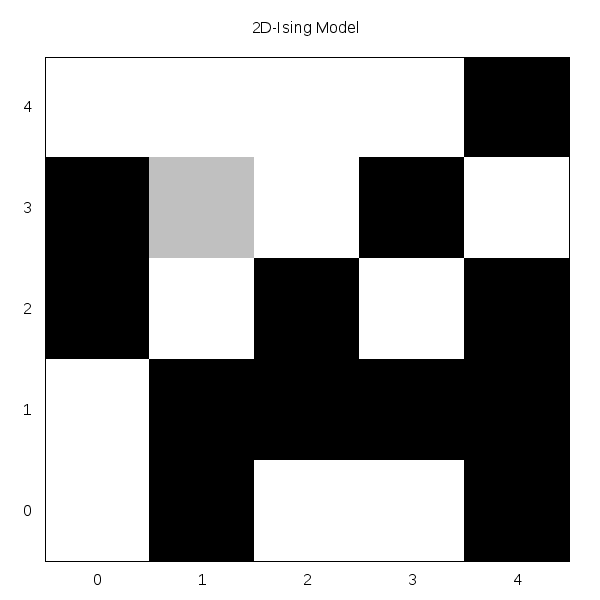
\includegraphics[width=0.5\textwidth]{../Graph_Export/cluster_veranschaulichung/Abbildung42.png} 
    \caption{}
  \end{minipage}
  \begin{minipage}[b]{6 cm}
    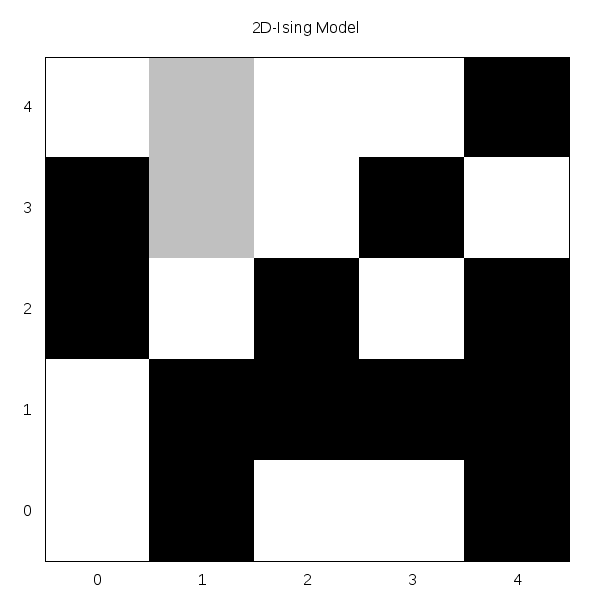
\includegraphics[width=0.5\textwidth]{../Graph_Export/cluster_veranschaulichung/Abbildung43a.png} 
    \caption{}
  \end{minipage}
  \begin{minipage}[b]{6 cm}
    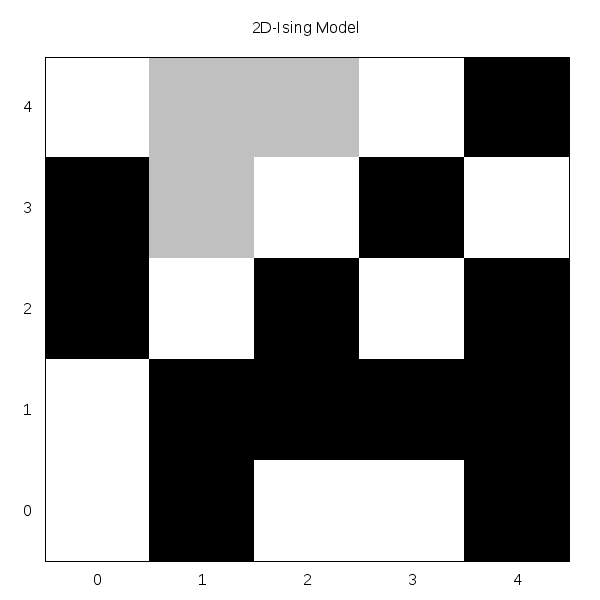
\includegraphics[width=0.5\textwidth]{../Graph_Export/cluster_veranschaulichung/Abbildung43b.png} 
    \caption{}
  \end{minipage}
  \begin{minipage}[b]{6 cm}
    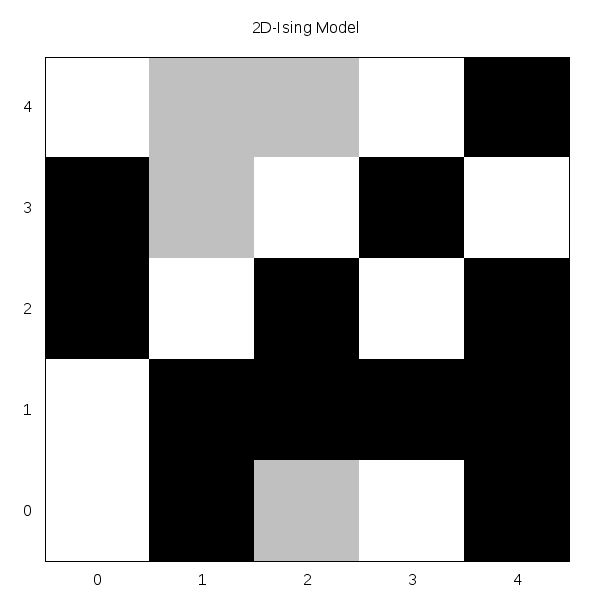
\includegraphics[width=0.5\textwidth]{../Graph_Export/cluster_veranschaulichung/Abbildung43c.png} 
    \caption{}
  \end{minipage}
\begin{minipage}[b]{6 cm}
    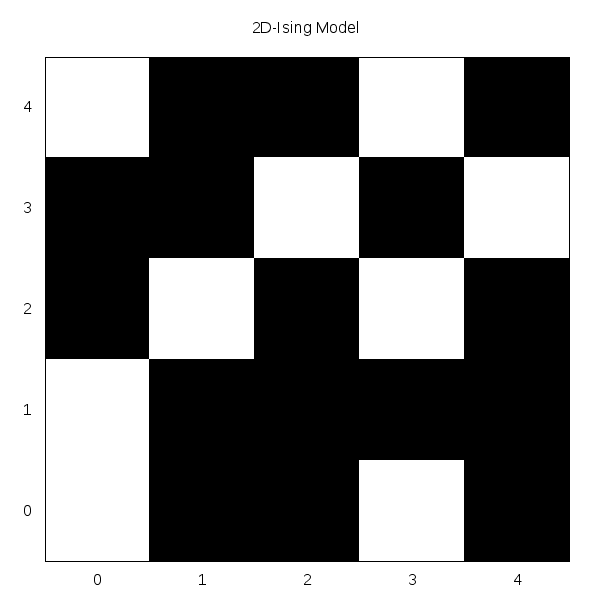
\includegraphics[width=0.5\textwidth]{../Graph_Export/cluster_veranschaulichung/Abbildung44.png} 
    \caption{}
  \end{minipage}
\end{figure}


\subsection{Flipp-Wahrscheinlichkeit des Clusters = 1}
Der Algorithmus wird besonders effizient, da bei einer bestimmten Annahme-Wahrscheinlichkeit p, dass ein Zustand in den Cluster aufgenommen wird, der Cluster in jedem Monte-Carlo-Schritt geflippt wird.\\\\
Warum dies so ist wird klar, wenn man sich die Wahrscheinlichkeit $W_{ij}$ für den Übergang von der Konfiguration i zu j berechnet.
\begin{align}
W_{ij} = min\{1, \frac{P_j}{P_i} \} = min\{1, \frac{A(j \rightarrow i) * P_j}{A(i \rightarrow j) * P_i} \} = min\{1, \frac{A(j \rightarrow i) * e^{-\beta E_j}}{A(i \rightarrow j) * e^{-\beta E_i}} \}
\end{align}
Für die Wahrscheinlichkeit $A(i \rightarrow j)$ den Übergang von i nach j zu betrachten und für die Energie $E_i$ im Zustand i gelten:\\
(Hierbei bedeutet $_{innen}$ jeweils innerhalb und $_{außen}$ außerhalb des Clusters\\
und $n_{gleich}$ bzw. $n_{diff}$ sind die Anzahl Spins, die am Rand gleich bzw. ungleich zu dem Spin innerhalb des Clusters sind.)
\begin{align}
A(i \rightarrow j)=A_{innen} * (1 - p)^{n_{gleich}}\\
A_{innen} = p^{n_{innen}-1} + Z\\
E_i = E_{innen} + E_{außen} - n_{gleich} * J + n_{diff} * J\\
\end{align}
Mit Z der Wahrscheinlichkeit einen Spin im Cluster als Startpunkt gewählt zu haben.\\
Ebenso gilt:
\begin{align}
A(j \rightarrow i)=A_{innen} * (1 - p)^{n_{diff}}\\
E_j = E_{innen} + E_{außen} + n_{gleich} * J - n_{diff} * J\\
\end{align}
Damit gilt:
\begin{align}
W_{ij} = min\{1, \frac{A_{innen}*(1-p)^{n_{diff}}}{A_{innen}*(1-p)^{n_{gleich}}} * \frac{e^{-\beta E_{innen} + E_{außen} + n_{gleich} * J - n_{diff} * J}}{e^{-\beta E_{innen} + E_{außen} - n_{gleich} * J + n_{diff} * J}}\}\\
= min\{1, \frac{(1-p)^{n_{diff}}}{(1-p)^{n_{gleich}}} * \frac{e^{-\beta n_{gleich} * J} * e^{+\beta n_{diff} * J}}{e^{+\beta n_{gleich} * J} * e^{-\beta n_{diff} * J}}\}\\
= min\{1, \frac{(1-p)^{n_{diff}}}{(1-p)^{n_{gleich}}} * \frac{e^{-2\beta n_{gleich} * J}}{e^{-2\beta n_{diff} * J}}\}\\
= min\{1, \left(\frac{(1-p)}{e^{-2\beta J}}\right)^{n_{diff}} * \left(\frac{e^{-2\beta J}}{(1-p)}\right)^{n_{gleich}}\}
\end{align}
Hieraus lässt sich nun erkennen, dass die Wahrscheinlichkeit vom Zustand i zu j überzugehen gleich $1$ wird, wenn wir $p = 1 - e^{-2\beta J}$ wählen.

\subsection{Konvergenzverhalten im Vergleich}
Der Vorteil des Cluster-Algorithmus ist die schnelle Konverenzgeschwindigkeit in der Nähe des Phasenübergangs bzw. der kritischen Temperatur.\\\\
(Graphen)\\\\
Wie man in Abbilddung 5.1 erkennt...\\